\documentclass[11pt, onecolumn, compsoc, letterpaper]{article}


% Usual setup packages
\usepackage{times}
\usepackage[utf8]{inputenc} % set input encoding (not needed with XeLaTeX)
\usepackage[margin=2.75cm]{geometry} % to change the page dimensions
\usepackage{graphicx} % General page control package
\usepackage[compact]{titlesec} % For compact title
\usepackage{listings} % For including source code with highlighting
\usepackage{subfiles} % For better multiple file per paper handling
\usepackage{hyperref} % For better hyper-link integration

% Packages for verbatim text blocks
\usepackage{alltt} % Package for including math in verbatim text
\usepackage{fancyvrb}

% Packages for math symbols and other mathey things
\usepackage{amsmath}
\usepackage{amsfonts}
\usepackage{amssymb}
\usepackage{mathtools}

% Packages for including pseudo-code
\usepackage{algorithmicx}
\usepackage{algorithm}
\usepackage{algpseudocode}

% Packages that handle lists
\usepackage{enumerate} % For reduced enumeration spacing
%\usepackage{enumitem} % For suppressing bullets
\usepackage{mdwlist} % Better control of lists

% Packages that handle tables, figures and other floats
\usepackage{tabularx}
\usepackage{multirow}
\usepackage{titling}
\usepackage{float} % To make floats movable
\usepackage[font=scriptsize,labelfont=bf]{caption}
\usepackage[font=scriptsize,labelfont=bf]{subcaption}
\usepackage{hhline}
\usepackage[usenames,dvipsnames]{color}
\usepackage[table]{xcolor}

% Packages for drawing graphs, FSMs, etc.
\usepackage{pgf}
\usepackage{tikz}
\usepackage{tikz-qtree}
\usetikzlibrary{shapes,arrows,calc,fit,positioning,shapes.symbols,shapes.callouts,patterns,automata}

% clean up references
\hypersetup{
    colorlinks,
    citecolor=black,
    filecolor=black,
    linkcolor=black,
    urlcolor=black
}

% smaller tab space
\lstset{
	tabsize=4
}

%%% HEADERS & FOOTERS
\usepackage{titlepic}
\usepackage{fancyhdr} % This should be set AFTER setting up the page geometry
\pagestyle{fancy} % options: empty , plain , fancy
\renewcommand{\headrulewidth}{0pt} % customise the layout...
\lhead{}\chead{}\rhead{}
\lfoot{}\cfoot{\thepage}\rfoot{}

%%% SECTION TITLE APPEARANCE
%\usepackage{sectsty}
%\allsectionsfont{\sffamily\mdseries\upshape} % (See the fntguide.pdf for font help)
% (This matches ConTeXt defaults)

%%% ToC (table of contents) APPEARANCE
%\usepackage[nottoc,notlof,notlot]{tocbibind} % Put the bibliography in the ToC
%\usepackage[titles,subfigure]{tocloft} % Alter the style of the Table of Contents
%\renewcommand{\cftsecfont}{\rmfamily\mdseries\upshape}
%\renewcommand{\cftsecpagefont}{\rmfamily\mdseries\upshape} % No bold!

% Nice Little macro for adding a comment box. Includes incrementing comment numbers.
\newcounter{comcount}
\setcounter{comcount}{0}
\newcommand{\mycomment}[1]
{
\refstepcounter{comcount}
\smallskip\noindent\fbox{\parbox{\linewidth}{\emph{Comment \arabic{comcount}} : \small{#1}}} 
}

% Math commands
\newcommand{\vnorm}[1]{\left|\left|#1\right|\right|}
\newcommand{\tab}{\hspace*{2em}}
\DeclareMathOperator*{\argminop}{arg\,min\,}
\DeclareMathOperator*{\argmaxop}{arg\,max\,}
\DeclarePairedDelimiter\ceil{\lceil}{\rceil}
\DeclarePairedDelimiter\floor{\lfloor}{\rfloor}
\newcommand{\argmin}[1]{\underset{#1}{\argminop}}
\newcommand{\argmax}[1]{\underset{#1}{\argmaxop}}
\newcommand{\D}[2]{\frac{d#1}{d#2}}
\newcommand{\PD}[2]{\frac{\partial #1}{\partial #2}}
\newcommand{\V}[1]{\mathbf{#1}}
\newcommand{\ubar}[1]{\underline{#1}}
\newcommand{\Ac}{\mathcal{A}} % (Bayesian) Action Profile
\newcommand{\St}{\mathcal{S}} % (Bayesian/Extensive) State List, Strategy set
\newcommand{\Pl}{\mathcal{N}} % (Extensive/Bayesian) Player List
\newcommand{\Hi}{\mathcal{H}} % (Extensive) Game History
\newcommand{\Pf}{\mathcal{P}} % (Extensive) Player Function
\newcommand{\Th}{\mathcal{Z}} % (Extensive) Terminal History
\newcommand{\Ta}{\mathcal{T}} % (Cooperative) Targets/Resources
\newcommand{\Co}{\mathcal{C}} % (Cooperative) Player assignment constraints

% Squeeze whitespace
\setlength{\parskip}{0pt}
\setlength{\parsep}{0pt}
\setlength{\headsep}{0pt}
\setlength{\topskip}{0pt}
\setlength{\topmargin}{0pt}
\setlength{\topsep}{0pt}
\setlength{\partopsep}{0pt}

\titlespacing{\section}{0pt}{*3}{*3}
\titlespacing{\subsection}{0pt}{*2}{*2}
\titlespacing{\subsubsection}{0pt}{*1}{*1}

\renewcommand{\arraystretch}{1.2}
\setlength{\droptitle}{-2cm}

\title{Performance Bounds on Distributed Target Assignment with Constraints}
\author{Anshul Kanakia}
\date{}

\begin{document}
\maketitle

\begin{abstract}
Target assignment is a well studied problem in the fields of game theory and optimization where a number of agents are assigned to a number of targets for maximum system welfare. For example, given a set of search/surveillance zones and a swarm of UAVs, this problem describes how the UAVs should be delegated to search zones so as to maximize some global welfare for the system. An extension of this problem is where each search zone require a minimum number of agents to be assigned to it to receive any payoff whatsoever. Another natural extension arises when certain agents cannot be assigned to specific search areas for a number of reasons such as fuel constraints, obstacles, environmental hazards, etc. We look at both these extensions and frame the problem of target threshold assignment with agent constraints as a communal welfare game and discuss distributed solutions to this problem.
\end{abstract}

%%%%%%%%%%%%%%%%%%%%%%%%%%%%%%%%%%%%%%%%%%%%%%%%%%%%%%%%%%%%%%%%%%%%%%%%%%%%%%%%
\section{Introduction}
We inspect the cooperative, distributed welfare game of vehicle-target assignment with welfare functions that are not sub-modular, but are instead based on target specific threshold values and player-target assignment constraints. Target threshold values define global system welfare based on the number of agents assigned to a target.  One can imagine cooperative scenarios where a group must attain at least some minimum size to successfully complete a task. Tasks such as real-time mapping, object detection, hazard containment, etc. fall into this category. Such tasks can often be seen as a special flavor of the vehicle-target assignment problem where agent groups of a certain size must pick the same target to successfully complete their mission and receive a non-zero payoff.

Such scenarios are prevalent in the fields of multi-agent systems and swarm robotics where large groups of individually simple agents must cooperate in order to complete complex tasks. Foraging, collective inspection, collective object detection and real-time mapping of a target perimeter (such as oil spills, forest fires etc.) are examples of situations where such a cooperative game approach is beneficial. 


%%%%%%%%%%%%%%%%%%%%%%%%%%%%%%%%%%%%%%%%%%%%%%%%%%%%%%%%%%%%%%%%%%%%%%%%%%%%%%%%
\section{Related Work}
Most recent work in distributed welfare games\cite{Marden2008, Marden2013} assumes that players are, in general, non-cooperative. While a comprehensive study of the vehicle-target assignment problem has been done by Arslan et al.\cite{Arslan2007}, the authors do not discuss the specific scenario discussed in this paper.

Since target thresholds remove the submodularity property from welfare functions for this game, work on valid utility games by Vetta et al.\cite{Vetta2002} cannot be used in this circumstance and additional analysis must be done to predict bounds on PoA/PoS.


%%%%%%%%%%%%%%%%%%%%%%%%%%%%%%%%%%%%%%%%%%%%%%%%%%%%%%%%%%%%%%%%%%%%%%%%%%%%%%%%
\section{Game Setup and Example}
The cooperative game is set up as follows:
\begin{itemize}
	\item Players: $\Pl = \{1,2,3,\ldots, N\}$.
	\item Targets: $t \in \Ta$, $|\Ta| = M$.
	\item Target Threshold: $k_t$, $t \in \Ta$.
	\item Player Constraints: $c_i = S \subseteq \Ta$, $c_i \in C$.
	\item Target Detection Probability: We assume all players can perfectly detect and assign themselves to targets within their constraints, $c_i$. Therefore detection probability for all targets is 1.
	\item Target specific welfare function, 
\begin{align}
	W_t(|a|_t) & = \left\{
	\begin{array}{ll}
		1 & |a|_t \geq k_t\\
		0 & o/w
	\end{array}\right.\label{eq:wf}
\end{align}
	\item Global welfare function,
\begin{align}
	W(a) = \sum\limits_{t \in \Ta} W_t(|a|_t)\label{eq:gwf}
\end{align}
\end{itemize}
We can clearly see that the welfare function, $W(|a|_t)$, is not submodular. The fact that the global welfare function is just an accumulator of ``successfully assigned'' targets does help with PoA/PoS analysis.

\textbf{Definition:} A target is considered ``successfully assigned'' when $|a|_t \geq k_t$, i.e. the number of player's assigned to it is greater than or equal to its threshold value.

\textbf{Definition:} A target is considered ``perfectly assigned'' when $|a|_t = k_t$.

The following example describes a cooperative game with target thresholds and player constraints as seen in Figure \ref{fig:ex1}.
\begin{itemize}
	\item Players: $\Pl = \{1,2,3,4\}$
	\item Targets: $t \in \Ta = \{a, b, c\}$
	\item Target Threshold: $k_a = k_b = k_c = 2$
	\item Target specific welfare function, $W_t(|a|_t)$, from \eqref{eq:wf}
	\item Anonymous Global welfare function, $W(a) = \sum\limits_{t \in \Ta} W_t(|a|_t)$, from \eqref{eq:gwf}.
\end{itemize}
\begin{figure}[!htb]
	\centering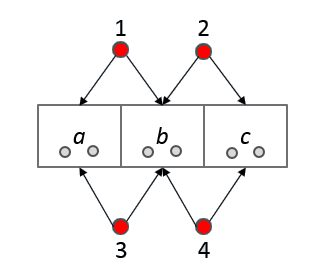
\includegraphics[width=5.5cm]{assets/ex1.png}
	\centering\caption{A cooperative game with 4 players and 3 targets. Gray pegs indicate the target's minimum threshold value while the arrows depict player assignment constraints.}\label{fig:ex1}
\end{figure}

Global welfare values for this example are listed in Table \ref{tab:mcgw}. Note that these values depend only on the number of successfully assigned targets. 
\begin{table}[!htb]
	\centering\begin{tabular}{r|c|c|}
	\multicolumn{1}{c}{}
	& \multicolumn{1}{c}{b}
	& \multicolumn{1}{c}{$c$}\\
	\cline{2-3}
	$a$ & $2$ & $1$\\
	\cline{2-3}
	$b$ & $1$ & $1$\\
	\cline{2-3}
	\multicolumn{1}{c}{}
	& \multicolumn{2}{c}{$a,b$}
	\end{tabular}~
	\centering\begin{tabular}{r|c|c|}
	\multicolumn{1}{c}{}
	& \multicolumn{1}{c}{$b$}
	& \multicolumn{1}{c}{$c$}\\
	\cline{2-3}
	$a$ & $1$ & $2$\\
	\cline{2-3}
	$b$ & $1$ & $1$\\
	\cline{2-3}
	\multicolumn{1}{c}{}
	& \multicolumn{2}{c}{$a,c$}
	\end{tabular}~
	\centering\begin{tabular}{r|c|c|}
	\multicolumn{1}{c}{}
	& \multicolumn{1}{c}{$b$}
	& \multicolumn{1}{c}{$c$}\\
	\cline{2-3}
	$a$ & $1$ & $1$\\
	\cline{2-3}
	$b$ & $1$ & $1$\\
	\cline{2-3}
	\multicolumn{1}{c}{}
	& \multicolumn{2}{c}{$b,b$}
	\end{tabular}~
	\centering\begin{tabular}{r|c|c|}
	\multicolumn{1}{c}{}
	& \multicolumn{1}{c}{$b$}
	& \multicolumn{1}{c}{$c$}\\
	\cline{2-3}
	$a$ & $1$ & $1$\\
	\cline{2-3}
	$b$ & $1$ & $2$\\
	\cline{2-3}
	\multicolumn{1}{c}{}
	& \multicolumn{2}{c}{$b,c$}
	\end{tabular}
	\centering\caption{Global welfare for the vehicle-target assignemt example scenario with target thresholds and player constraints.}\label{tab:mcgw}
\end{table}

\section{Possible Scenarios}
\subsection{Case I: True target thresholds are known to all agents}


%%%%%%%%%%%%%%%%%%%%%%%%%%%%%%%%%%%%%%%%%%%%%%%%%%%%%%%%%%%%%%%%%%%%%%%%%%%%%%%%
\section{Selecting Utility Functions}
We discuss the effects that choosing different utility functions has for this example scenario. We discuss two utility functions, marginal contribution and Shapley value utility, and apply log-linear learning to observe equilibria of the system under both utility design choices.

\subsection{Marginal Contribution (MC) Utility}
MC utility gives us two important and desirable properties for a good utility function, existence and efficiency of NE. NE existence is guaranteed because the chosen binary welfare function is anonymous and  depends only on the number of vehicles assigned to a target\cite{Monderer1996}. Given that the global objective function is just a counting function that counts the total number of successfully assigned targets, we can show that a maximum assignment is always an NE of the system as it results in maximum player payoffs (see proof in \textbf{Price of Stability} section). Player utility values using MC utility are listed in Table \ref{tab:mcUtil}.  

\begin{table}[!htb]
	\centering\begin{tabular}{r|c|c|}
	\multicolumn{1}{c}{}
	& \multicolumn{1}{c}{b}
	& \multicolumn{1}{c}{$c$}\\
	\cline{2-3}
	$a$ & \textcolor{blue}{$1,1,1,1$} & $1,1,0,0$\\
	\cline{2-3}
	$b$ & $0,0,0,0$ & \textcolor{red}{$1,0,0,1$}\\
	\cline{2-3}
	\multicolumn{1}{c}{}
	& \multicolumn{2}{c}{$a,b$}
	\end{tabular}~
	\centering\begin{tabular}{r|c|c|}
	\multicolumn{1}{c}{}
	& \multicolumn{1}{c}{$b$}
	& \multicolumn{1}{c}{$c$}\\
	\cline{2-3}
	& $1,0,1,0$ & \textcolor{blue}{$1,1,1,1$}\\
	\cline{2-3}
	& \textcolor{red}{$1,1,0,0$} & $0,1,0,1$\\
	\cline{2-3}
	\multicolumn{1}{c}{}
	& \multicolumn{2}{c}{$a,c$}
	\end{tabular}~
	\centering\begin{tabular}{r|c|c|}
	\multicolumn{1}{c}{}
	& \multicolumn{1}{c}{$b$}
	& \multicolumn{1}{c}{$c$}\\
	\cline{2-3}
	& $0,0,0,0$ & \textcolor{red}{$0,0,1,1$}\\
	\cline{2-3}
	& \textcolor{red}{$0,0,0,0$} & $0,0,0,0$\\
	\cline{2-3}
	\multicolumn{1}{c}{}
	& \multicolumn{2}{c}{$b,b$}
	\end{tabular}~
	\centering\begin{tabular}{r|c|c|}
	\multicolumn{1}{c}{}
	& \multicolumn{1}{c}{$b$}
	& \multicolumn{1}{c}{$c$}\\
	\cline{2-3}
	& \textcolor{red}{$0,1,1,0$} & $0,1,0,1$\\
	\cline{2-3}
	& $0,0,0,0$ & \textcolor{blue}{$1,1,1,1$}\\
	\cline{2-3}
	\multicolumn{1}{c}{}
	& \multicolumn{2}{c}{$b,c$}
	\end{tabular}
	\centering\caption{Player payoffs for the example scenario using Marginal Contribution utility.}\label{tab:mcUtil}
\end{table}

Averaging over 1000 runs of log-linear learning for 1000 iterations each and using temperature $T = 0.15$, the following stationary distribution is observed (Table \ref{tab:mcsd}).

\begin{table}[!htb]
	\centering\begin{tabular}{r|c|c|}
	\multicolumn{1}{c}{}
	& \multicolumn{1}{c}{b}
	& \multicolumn{1}{c}{$c$}\\
	\cline{2-3}
	$a$ & \textcolor{blue}{$0.343$} & $0.000$\\
	\cline{2-3}
	$b$ & $0.002$ & \textcolor{red}{$0.000$}\\
	\cline{2-3}
	\multicolumn{1}{c}{}
	& \multicolumn{2}{c}{$a,b$}
	\end{tabular}~
	\centering\begin{tabular}{r|c|c|}
	\multicolumn{1}{c}{}
	& \multicolumn{1}{c}{$b$}
	& \multicolumn{1}{c}{$c$}\\
	\cline{2-3}
	& $0.001$ & \textcolor{blue}{$0.308$}\\
	\cline{2-3}
	& \textcolor{red}{$0.000$} & $0.000$\\
	\cline{2-3}
	\multicolumn{1}{c}{}
	& \multicolumn{2}{c}{$a,c$}
	\end{tabular}~
	\centering\begin{tabular}{r|c|c|}
	\multicolumn{1}{c}{}
	& \multicolumn{1}{c}{$b$}
	& \multicolumn{1}{c}{$c$}\\
	\cline{2-3}
	& $0.000$ & \textcolor{red}{$0.001$}\\
	\cline{2-3}
	& \textcolor{red}{$0.000$} & $0.000$\\
	\cline{2-3}
	\multicolumn{1}{c}{}
	& \multicolumn{2}{c}{$b,b$}
	\end{tabular}~
	\centering\begin{tabular}{r|c|c|}
	\multicolumn{1}{c}{}
	& \multicolumn{1}{c}{$b$}
	& \multicolumn{1}{c}{$c$}\\
	\cline{2-3}
	& \textcolor{red}{$0.000$} & $0.000$\\
	\cline{2-3}
	& $0.000$ & \textcolor{blue}{$0.345$}\\
	\cline{2-3}
	\multicolumn{1}{c}{}
	& \multicolumn{2}{c}{$b,c$}
	\end{tabular}
	\centering\caption{Stationary Distribution approximated using log-linear learning and MC utility.}\label{tab:mcsd}
\end{table}

As is evident from these results, applying log-linear learning using MC utility converges the system to perfect target assignment if a perfect assignment can be made. The NE in blue are all cases of perfect assignment while the equilibria in red are cases of successful assignment but do not maximize global welfare. We now look at what happens when Shapley value utility is used instead of MC for this game.

\subsection{Shapley Value (SV) Utility}
Using SV utility, each player's utility for selecting target, $t \in \Ta$, can be computed using the simplified equation,
\begin{align}
	U_i(t, a_{-i}) & = \left\{
		\begin{array}{ll}	
			1/|a|_t & |a|_t \geq k_t\\
			0 & |a|_t < k_t
		\end{array}\right.
\end{align}

Player utility values are listed in Table \ref{tab:svUtil}. Once again, running log-linear learning with the same parameters as used for marginal contribution utility we see the following stationary distribution (Table \ref{tab:svsd}).
\begin{table}[!htb]
	\centering\begin{tabular}{r|c|c|}
	\multicolumn{1}{c}{}
	& \multicolumn{1}{c}{b}
	& \multicolumn{1}{c}{$c$}\\
	\cline{2-3}
	$a$ & \textcolor{blue}{$\frac{1}{2},\frac{1}{2},\frac{1}{2},\frac{1}{2}$} & $\frac{1}{2},0\frac{1}{2},0$\\
	\cline{2-3}
	$b$ & $\frac{1}{3},\frac{1}{3},0,\frac{1}{3}$ & \textcolor{red}{$\frac{1}{2},0,0,\frac{1}{2}$}\\
	\cline{2-3}
	\multicolumn{1}{c}{}
	& \multicolumn{2}{c}{$a,b$}
	\end{tabular}~
	\centering\begin{tabular}{r|c|c|}
	\multicolumn{1}{c}{}
	& \multicolumn{1}{c}{$b$}
	& \multicolumn{1}{c}{$c$}\\
	\cline{2-3}
	& $\frac{1}{2},0,\frac{1}{2},0$ & \textcolor{blue}{$\frac{1}{2},\frac{1}{2},\frac{1}{2},\frac{1}{2}$} \\
	\cline{2-3}
	& \textcolor{red}{$\frac{1}{2},\frac{1}{2},0,0$} & $0,\frac{1}{2},0\frac{1}{2}$ \\
	\cline{2-3}
	\multicolumn{1}{c}{}
	& \multicolumn{2}{c}{$a,c$}
	\end{tabular}~
	\centering\begin{tabular}{r|c|c|}
	\multicolumn{1}{c}{}
	& \multicolumn{1}{c}{$b$}
	& \multicolumn{1}{c}{$c$}\\
	\cline{2-3}
	& $0,\frac{1}{3},\frac{1}{3},\frac{1}{3}$ & \textcolor{red}{$0,0,\frac{1}{2},\frac{1}{2}$}\\
	\cline{2-3}
	& \textcolor{red}{$\frac{1}{4},\frac{1}{4},\frac{1}{4},\frac{1}{4}$} & $\frac{1}{3},0,\frac{1}{3},\frac{1}{3}$\\
	\cline{2-3}
	\multicolumn{1}{c}{}
	& \multicolumn{2}{c}{$b,b$}
	\end{tabular}~
	\centering\begin{tabular}{r|c|c|}
	\multicolumn{1}{c}{}
	& \multicolumn{1}{c}{$b$}
	& \multicolumn{1}{c}{$c$}\\
	\cline{2-3}
	& \textcolor{red}{$0,\frac{1}{2},\frac{1}{2},0$} & $0,\frac{1}{2},0,\frac{1}{2}$\\
	\cline{2-3}
	& $\frac{1}{3},\frac{1}{3},\frac{1}{3},0$ & \textcolor{blue}{$\frac{1}{2},\frac{1}{2},\frac{1}{2},\frac{1}{2}$}\\
	\cline{2-3}
	\multicolumn{1}{c}{}
	& \multicolumn{2}{c}{$b,c$}
	\end{tabular}
	\centering\caption{Player payoffs using Shapley Value utility.}\label{tab:svUtil}
\end{table}
\begin{table}[!htb]
	\centering\begin{tabular}{r|c|c|}
	\multicolumn{1}{c}{}
	& \multicolumn{1}{c}{b}
	& \multicolumn{1}{c}{$c$}\\
	\cline{2-3}
	$a$ & \textcolor{blue}{$0.175$} & $0.004$\\
	\cline{2-3}
	$b$ & $0.055$ & \textcolor{red}{$0.005$}\\
	\cline{2-3}
	\multicolumn{1}{c}{}
	& \multicolumn{2}{c}{$a,b$}
	\end{tabular}~
	\centering\begin{tabular}{r|c|c|}
	\multicolumn{1}{c}{}
	& \multicolumn{1}{c}{$b$}
	& \multicolumn{1}{c}{$c$}\\
	\cline{2-3}
	& $0.003$ & \textcolor{blue}{$0.159$}\\
	\cline{2-3}
	& \textcolor{red}{$0.004$} & $0.005$\\
	\cline{2-3}
	\multicolumn{1}{c}{}
	& \multicolumn{2}{c}{$a,c$}
	\end{tabular}~
	\centering\begin{tabular}{r|c|c|}
	\multicolumn{1}{c}{}
	& \multicolumn{1}{c}{$b$}
	& \multicolumn{1}{c}{$c$}\\
	\cline{2-3}
	& $0.057$ & \textcolor{red}{$0.002$}\\
	\cline{2-3}
	& \textcolor{red}{$0.266$} & $0.046$\\
	\cline{2-3}
	\multicolumn{1}{c}{}
	& \multicolumn{2}{c}{$b,b$}
	\end{tabular}~
	\centering\begin{tabular}{r|c|c|}
	\multicolumn{1}{c}{}
	& \multicolumn{1}{c}{$b$}
	& \multicolumn{1}{c}{$c$}\\
	\cline{2-3}
	& \textcolor{red}{$0.005$} & $0.004$\\
	\cline{2-3}
	& $0.056$ & \textcolor{blue}{$0.154$}\\
	\cline{2-3}
	\multicolumn{1}{c}{}
	& \multicolumn{2}{c}{$b,c$}
	\end{tabular}
	\centering\caption{Stationary Distribution approximated using log-linear learning and SV utility.}\label{tab:svsd}
\end{table}

In this case, the worst NE has the highest likelihood of being chosen by log-linear learning. The case when all the agents are assigned to the same target ($b, b, b, b$) results in both, minimum player utility as well as the lowest global welfare but is still an equilibrium of the game. While one can argue that the ``good'' equilibria---with equal global welfare and player payoffs---are collectively more likely to occur compared to the one bad equilibrium, this is still a $\approx 2:1 ((.175 + .159 + .154) / .266)$ ratio.

In this example case it is clearly a better idea to use MC over SV when picking an appropriate utility function for this system to do optimal target assignment.

%%%%%%%%%%%%%%%%%%%%%%%%%%%%%%%%%%%%%%%%%%%%%%%%%%%%%%%%%%%%%%%%%%%%%%%%%%%%%%%%
\section{Price of Anarchy/Price of Stability Analysis}
\subsection{Price of Anarchy (PoA)}
PoA for this game is only defined under specific conditions for this vehicle-target assignment problem. The global welfare for the worst NE of the game can be $W_{NE}^{bad} = 0$, e.g. $|\Pl| = 3$, $|\Ta| = 3$, $c_i = \Ta$ $\forall i \in \Pl$, $k_t = 3$ $\forall t \in \Ta$. If every agent is assigned a unique target in this situation, then the system is at an equilibrium and no agent has any incentive to unilaterally deviate since they cannot improve their respective payoff or the global system welfare. In such a situation $W_{NE} = 0$ and thus $PoA = W_{OPT} / W_{NE}^{bad}$ would be undefined (or infinite).

In general, $W_{NE}^{bad} \not= 0$ when: for all actions in the valid action set, there must exist a target-$t$ such that it is either successfully assigned or is one agent away from being successfully assigned and an agent-$p$ exists that is not assigned to $t$ in the current action but has $t$ in it's target constraint set ($t \in c_p$, $a_p \not= t$).
\begin{align}
	\forall a \in 2^\Co, \exists t \in \Ta \text{ s.t. } |a|_t \geq (k_t - 1)\label{eq:poa}
\end{align}

If the property \eqref{eq:poa} holds for a given game then its PoA is bounded; $1 \leq PoA \leq W_{OPT}$. As more agents are ``added'' to the game (effectively creating a new game), the PoA goes down from $W_{OPT}$ to 1 when $|\Pl| \geq \sum\limits_{t \in \Ta} k_t$ (see Figure \ref{fig:poa}).

\begin{figure}[!htb]
	\centering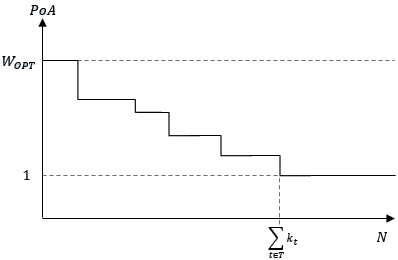
\includegraphics[width=7.5cm]{assets/poa.png}
	\centering\caption{Bounds on PoA as $|\Pl|$ increases.}\label{fig:poa}
\end{figure}

\subsection{Price of Stability (PoS)}
PoS for this game is always 1. To prove this, assume we start with an action $a^{OPT}$ which results in optimal global welfare $W_{OPT}$. I will prove that this action $a^{OPT}$ must also be NE$^{best}$. If a player decides to unilaterally deviate from $a^{OPT}$ to $a'$ then $U_i(a'_i, a'_{-i}) > U_i(a^{OPT}_i, a^{OPT}_{-i})$. This means that the target $a'_i$ must not have been optimally assigned for action $a^{OPT}$. It is easy to see that a player's utility can only be increased if they move between successfully assigned targets or from some target (not necessarily successfully assigned) to a successfully assigned target. This results in one of two scenarios, either target $a^{OPT}_i$ was successfully assigned before the switch and is no longer successfully assigned in action $a'$ or both targets $a^{OPT}_i$ and $a'_i$ are successfully assigned in $a'$. 

If the first case is true then that means target $a'_i$ was successfully assigned in action $a'$ by the switch from player-$i$ but was not successfully assigned in action $a^{OPT}$ (this is the only way player-$i$ could receive a better payoff for deviating from $a^{OPT}$). This means the global welfare is reduced by 1 and increased by one when going from $a^{OPT}$ to $a'$ which means $a'$ is another optimal action and we can replace our starting action with this new one and continue this recursive argument.

If the second case is true then player-$i$ switch did nothing to the global welfare and we can once again replace $a^{OPT}$ with $a'$ and continue this argument.

Finally, if this player's deviation from $a^{OPT}$ to $a'$ resulted in a better payoff for any other reason, it means the new target chosen $a'_i$ was not successfully assigned in action $a^{OPT}$ but has been successfully assigned in action $a'$. This would imply $W(a') > W(a^{OPT})$ since action $a'$ now has one new successfully assigned target, $a'_i$. This would result in a contradiction since that would imply $a^{OPT}$ was never an optimum. Which means that no player-$i$ would deviate from $a^{OPT}$ for any reason, thereby making $a^{OPT}$ a NE. $a^{OPT}$ is also the best NE, $W(a^{OPT}) = W_{NE}^{best}$ by it's very definition and so PoS for this game is always 1.



%%%%%%%%%%%%%%%%%%%%%%%%%%%%%%%%%%%%%%%%%%%%%%%%%%%%%%%%%%%%%%%%%%%%%%%%%%%%%%%%
\section{Finding Optimal Welfare}
Since the global welfare function is essentially a counting function (1 for targets that have been successfully assigned, 0 otherwise), it is maximized by maximizing the number of successfully assigned targets.

In the simplistic case when $k_t = k$ $\forall t \in \Ta$, and $c_i = \Ta$ $\forall i \in \Pl$, the maximum welfare is,
\begin{align}
	W^{OPT} & = \left\{
	\begin{array}{ll}
		\floor*{\frac{N}{k}} & M \geq N/k\\
		M & o/w
	\end{array}
	\right.\notag\\
	& = \min\left(\left\lfloor\frac{N}{k}\right\rfloor, M\right)
\end{align}

In the more complex case when $k_t$'s are not all the same value, the optimal welfare is found by maximizing the number of targets that can be successfully assigned. This is equivalent to a well studied problem in computer science called the \textbf{0-1 Integer Knapsack Problem} which, when posed as an optimization problem, is known to be NP-hard. This means that no polynomial time (in M) algorithm exists that can assign players to targets to maximize system utility---which makes finding $W^{OPT}$ and in turn, PoA/PoS for this game, a difficult problem for large values of $M$. For many practical purposes, a pseudo-polynomial time algorithm exists to solve the knapsack problem.

Finally, re-introducing player constraints makes finding $W_{OPT}$ an even more complicated affair and I have not studied this further, as yet. This would be a good future direction to take this preliminary work in.


%%%%%%%%%%%%%%%%%%%%%%%%%%%%%%%%%%%%%%%%%%%%%%%%%%%%%%%%%%%%%%%%%%%%%%%%%%%%%%%%
\section{Conclusion}
There are a number of further questions one can ask about the class of games discussed in this paper. My goal was mainly to show that game theory can be a viable alternative means to study cooperative scenarios with the system restrictions mentioned in this paper. While my bounds on PoA are not particularly satisfying, and rather obviously inferred just by thinking about such systems, perhaps a deeper analysis of the problem can provide exact values for PoA under special conditions\ldots Probably involving ratios between $|\Pl|$, $|\Ta|$ and $k_t$.

From the final section about finding the optimal global welfare for this class of games, I realized---to my amusement---that switching the problem around on it's head effectively invents a new method for solving the Knapsack Problem. All one has to do is define the knapsack problem as a cooperative game with target threshold values and performing log-linear learning on \emph{that} problem would give you an approximate solution to the original Knapsack problem!

As mentioned in the introduction, I find that this class of cooperative games definitely has a lot of potential for being a viable method for multi-agent, cooperative task design and analysis and should definitely be studied further.


% Bibliography
% \nocite{*} % Show all Bib-entries
\bibliographystyle{plainCustom}
\bibliography{refs}
\end{document}